\section{Mémoire distribuée - MPI}
Pour l'implémentation en mémoire distribuée, nous nous sommes concentrés sur le GEMM. Afin d'avoir une implémentation performante nous avons choisi 
d'implémenter le papier \textit{SUMMA: Scalable Universal Matrix Multipli cation Algorithm}\cite{SUMMA}. Nous avons donc réalisé une première version naïve de l'algorithme nous permettant
d'utiliser des communications collectives plutôt que des communications points à points. En effet, la base de notre code repose sur le partage des blocs à tous les processus
le nécessitant au travers d'une seule communication. Pour se faire on utilise un communicateur pour chaque ligne et chaque colonne de la matrice. Nous avons également décidé
de garder la distribution de la matrice donnée dans le projet. Les processus vont travailler localement sur la/les tuiles de la matrice C qu'ils possèdent. Ils vont réaliser
une accumulation sur cette partie au fur et à mesure que les lignes et colonnes nécessaires au traitement lui seront communiquées (via les communications collectives (broadcasts)).
Il y a deux phases distinctes dans la partie implémentée. La première correspond à la diffusion de la matrice B, où toutes les lignes de B nécessaires sont communiquées à tous les processus
sur la même colonne. Puis la diffusion de A se fait à tous les processus sur la même ligne, bloc par bloc, au fur et à mesure de l'avancée des sommes locales.

\begin{figure}
    \centering
    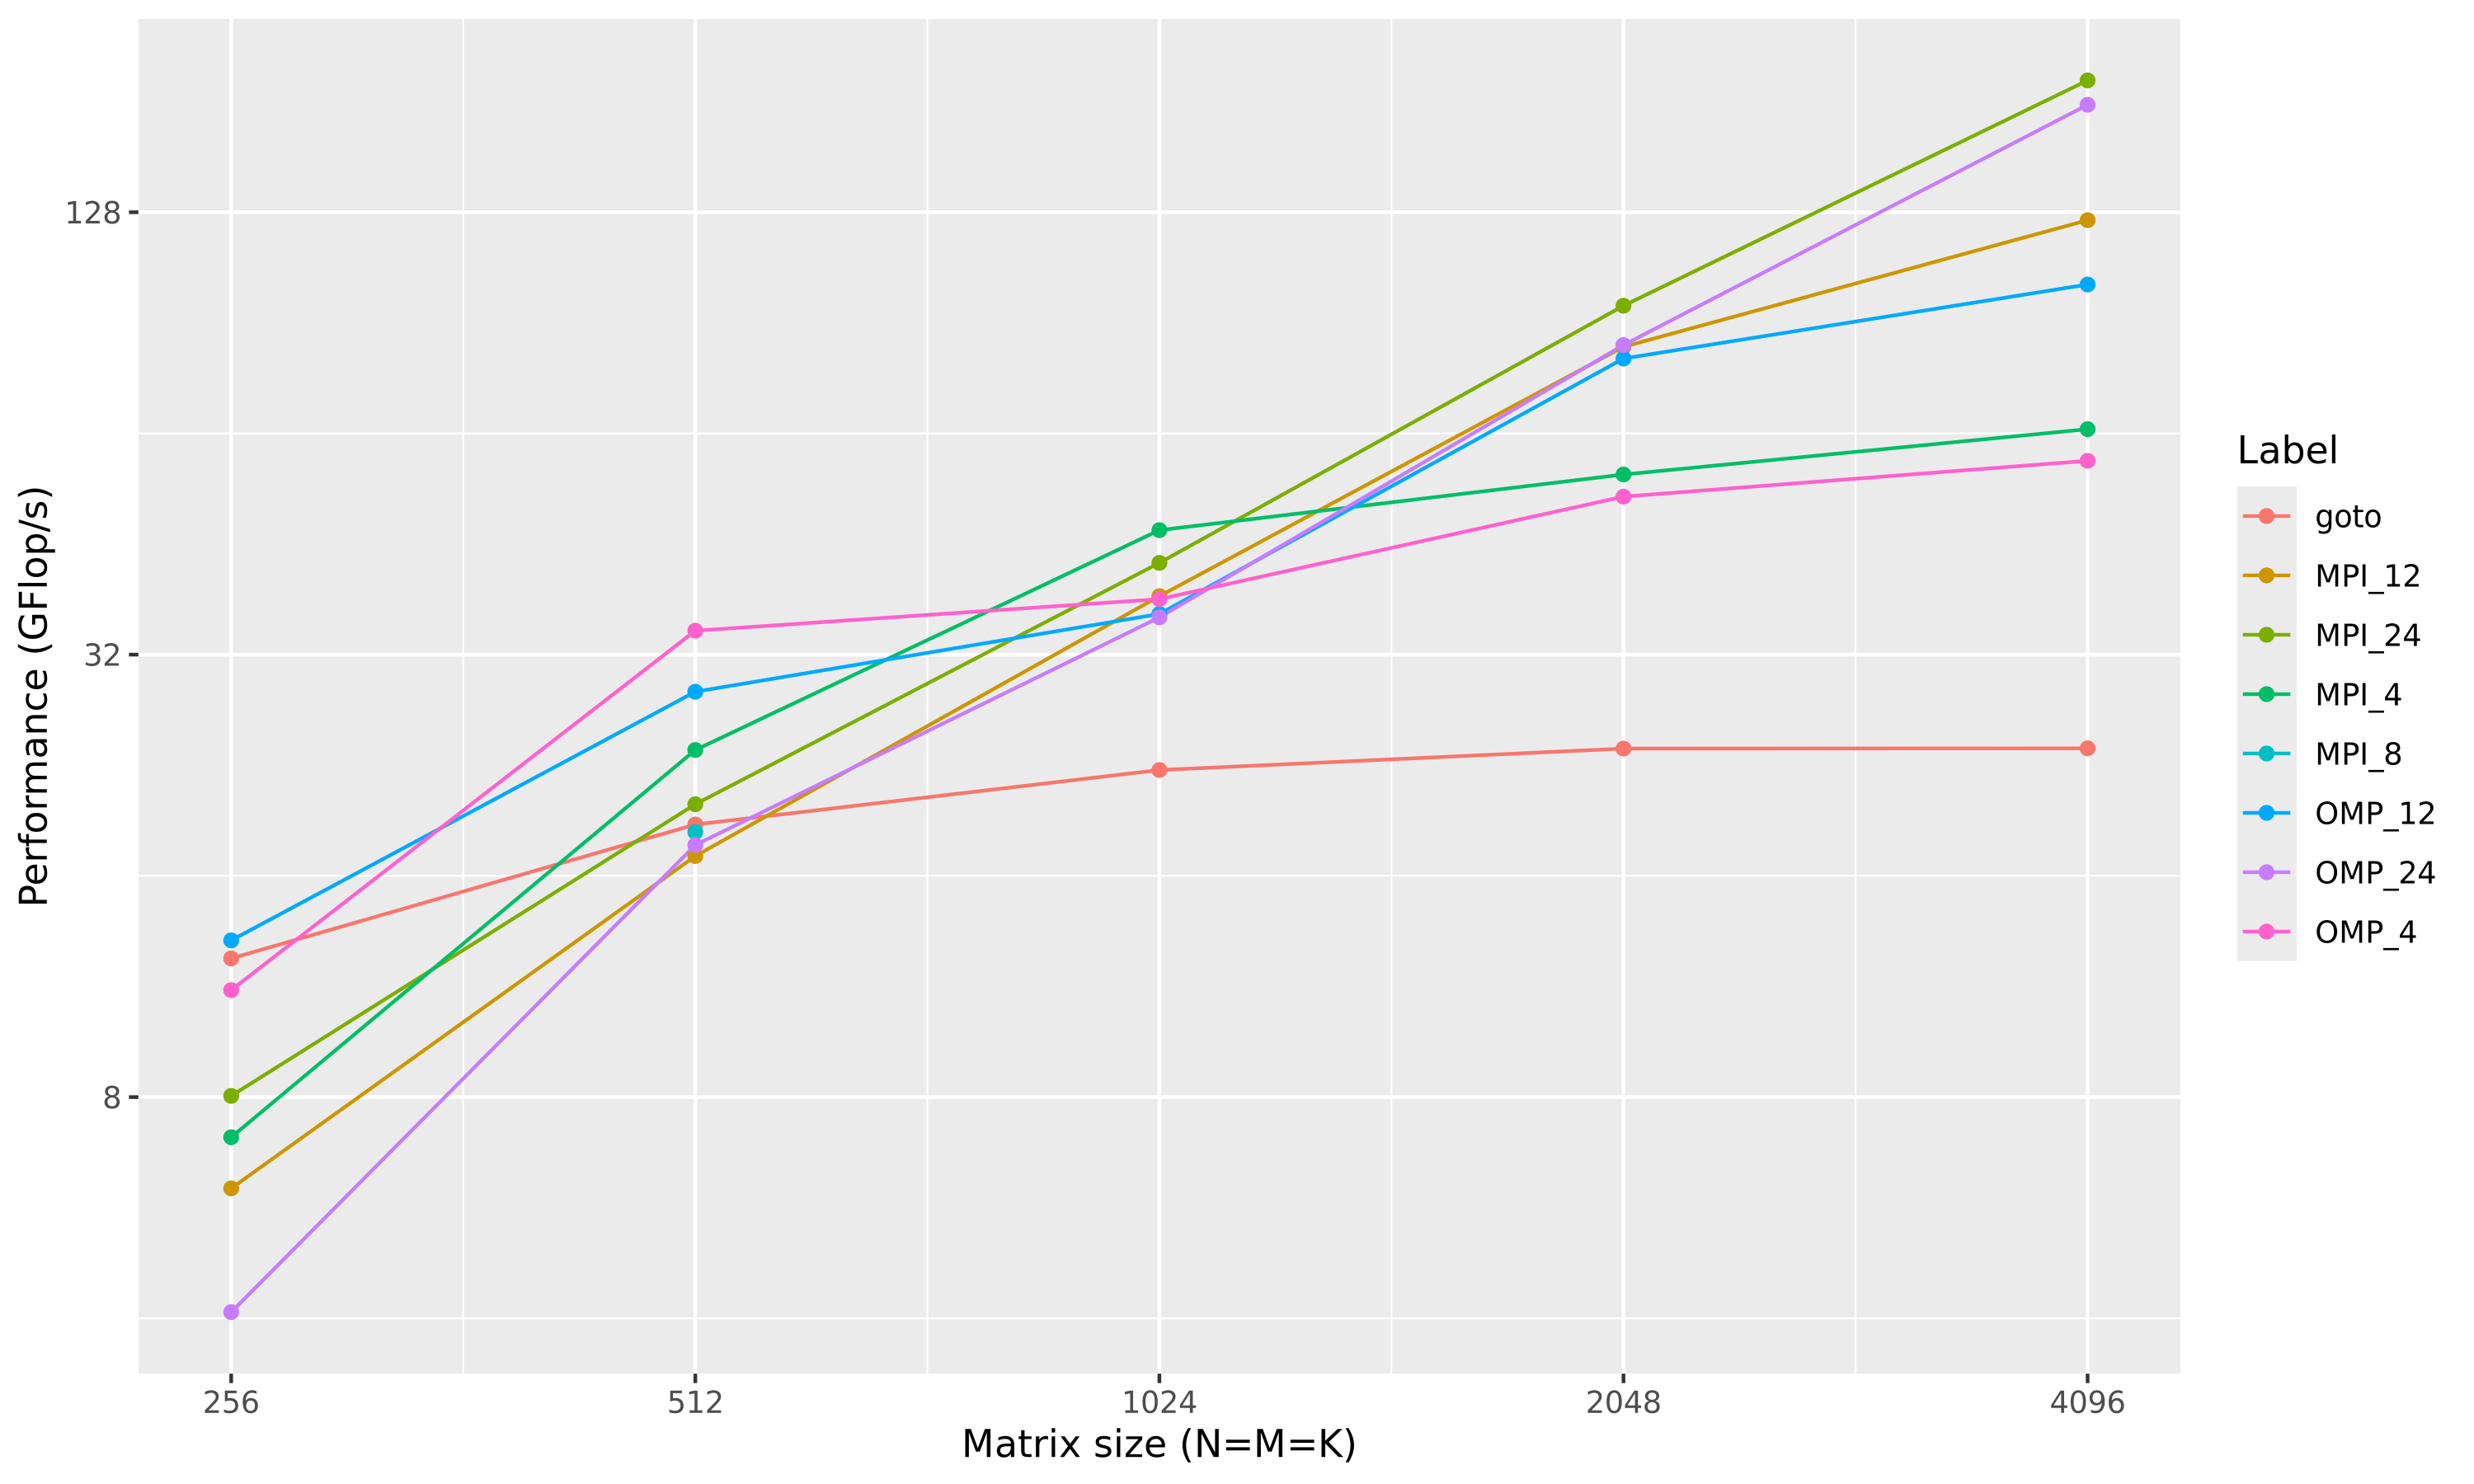
\includegraphics[width=0.8\textwidth]{assets/dgemm_mpi/MPI_vs_OMP.png}
    \caption{Comparaison des versions mémoire partagée et distribuée sur un nœud}
    \label{fig:mpi_omp}
\end{figure}


Nous avons ensuite commencé par effectuer des tests sur une machine pour comparer avec les versions mémoire partagée vues précédemment. Nous avons choisi de placer un processus
par banc NUMA afin de pouvoir limiter les accès aux mémoires plus éloignées en utilisant des communications MPI lorsque cela est nécessaire. On remarque sur la Figure \ref{fig:mpi_omp}, que cette 
version MPI semble obtenir les mêmes résultats que la version OpenMP naïve. Cependant les performances de cette version étant deux fois inférieures à celle utilisant le tuilage,
nous avons adapté notre version MPI pour qu'elle puisse utiliser la version tuilée OpenMP. Pour ce faire, il faut passer par un re-packing des matrices A,B et C, ce qui à un impact 
sur le nombre d'opérations supplémentaires à réaliser.

\begin{figure}
    \centering
    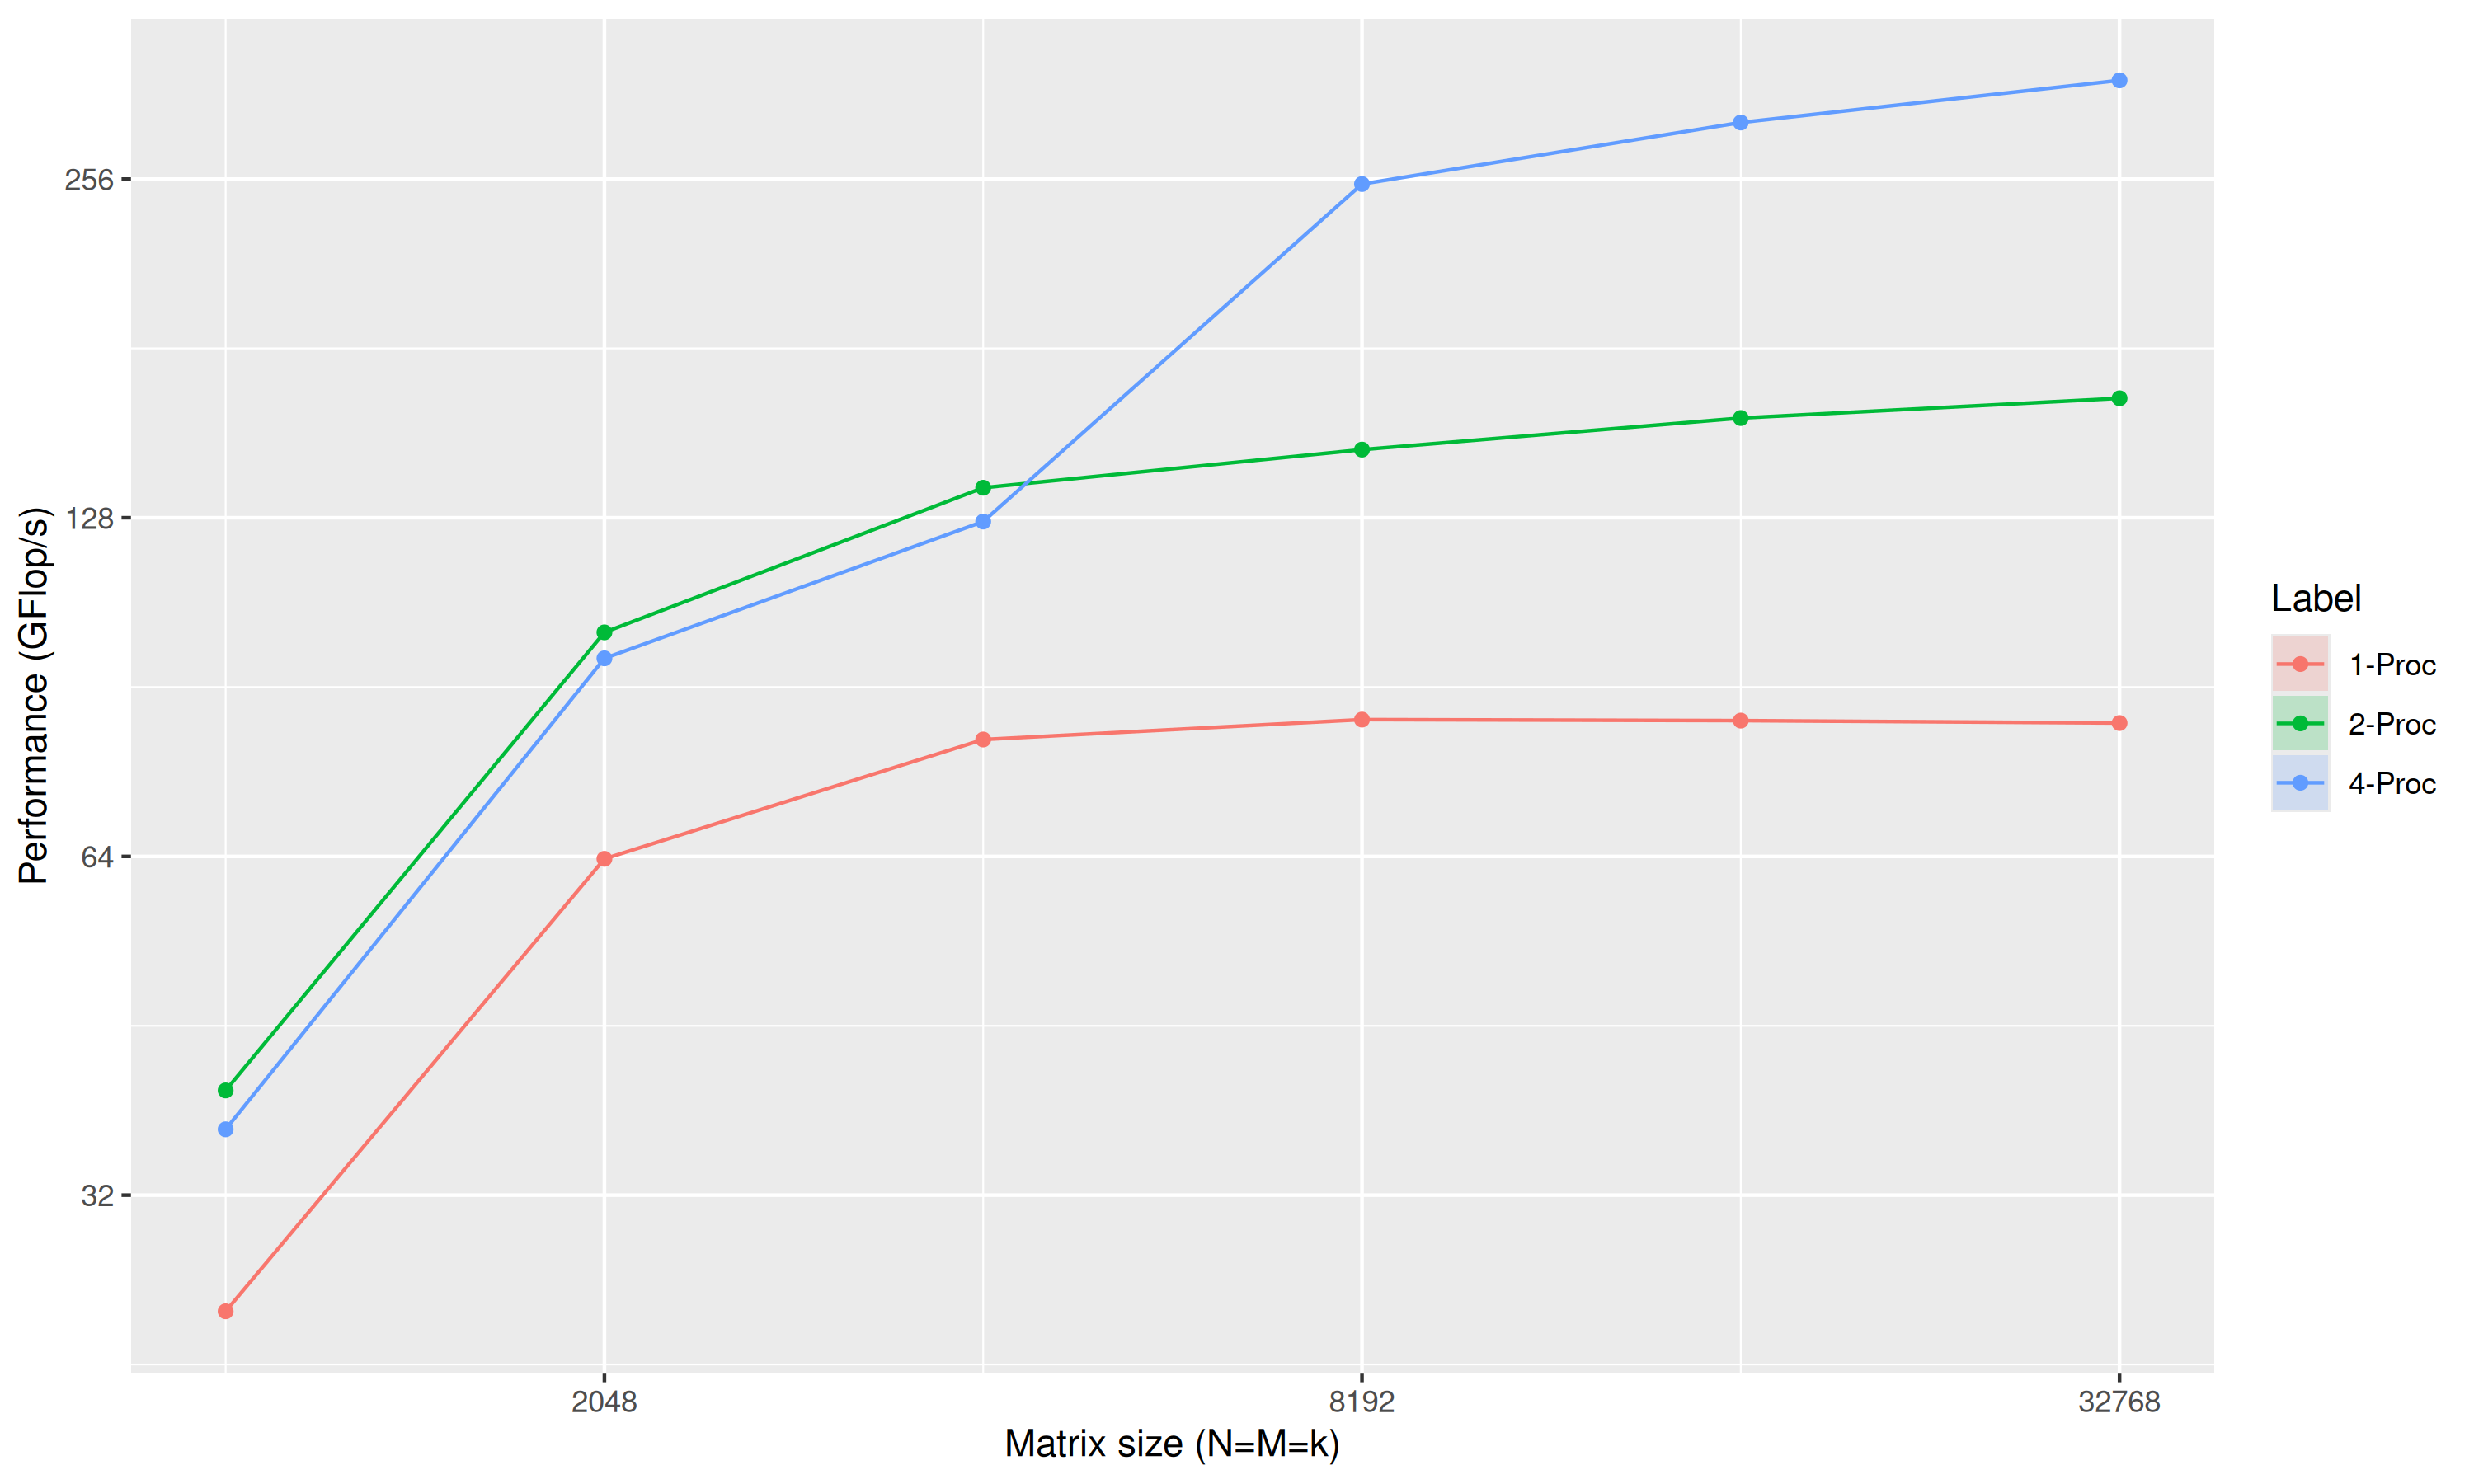
\includegraphics[width=0.8\textwidth]{assets/dgemm_mpi/strong_one_node.png}
    \caption{Test de scalabilité forte sur une seule machine (différents nombres de processus)}
    \label{fig:strong_one_node}
\end{figure}

Nous avons réalisé un test de scalabilité forte sur un nœud afin d'analyser la scalabilité sur une seule machine. La Figure \ref{fig:strong_one_node} permet de visualiser
ce test avec plusieurs nombres de processus actifs. Chaque processus utilise 6 threads, la version à 4 processus étant donc celle utilisant toute la machine. On remarque
d'abord que lorsque les matrices atteignent des tailles assez grandes ($>$4096x4096), on obtient une bonne scalabilité. En effet, les performances avec 4 processus
sont presque 4 fois supérieures à celles obtenues avec un seul ($\approx 84$ GFlop/s contre $\approx 310$ GFlop/s ce qui équivaut à une accélération d'environ x3.7).

L'objectif principal de cette version étant de réaliser une multiplication de matrices sur plusieurs nœuds, nous avons donc ensuite cherché quelle serait la taille optimale pour 
chaque tuile de nos matrices. Pour ce faire, nous avons utilsé les données vu dans la partie \ref{part:omp}. Puisque la taille de matrice pour laquelle nous nous
rapprochons le plus des performances de \textit{Cblas} est 4096x4096, nous avons choisi cette taille pour nos tuiles. De plus, si l'on regarde les performances avec un seul processus
sur la Figure \ref{fig:strong_one_node}, on voit que c'est également pour cette taille que l'on semble avoir atteint un palier avant de stagner puis de décroitre. Après avoir fixé la taille des tuiles,
nous avons étudié la scalabilité forte de nos deux versions. Nous sommes restés sur des matrices de taille maximale 65536x65536 afin de pouvoir réaliser un maximum de tests, que ce soit
pour pouvoir explorer le plus de paramètres possibles, mais également pour partager les ressources disponibles sur le cluster (notamment lorsque l'on utilise 8 machines).

\begin{figure}[htbp]
    \centering
    \begin{minipage}{0.48\textwidth}
        \centering
        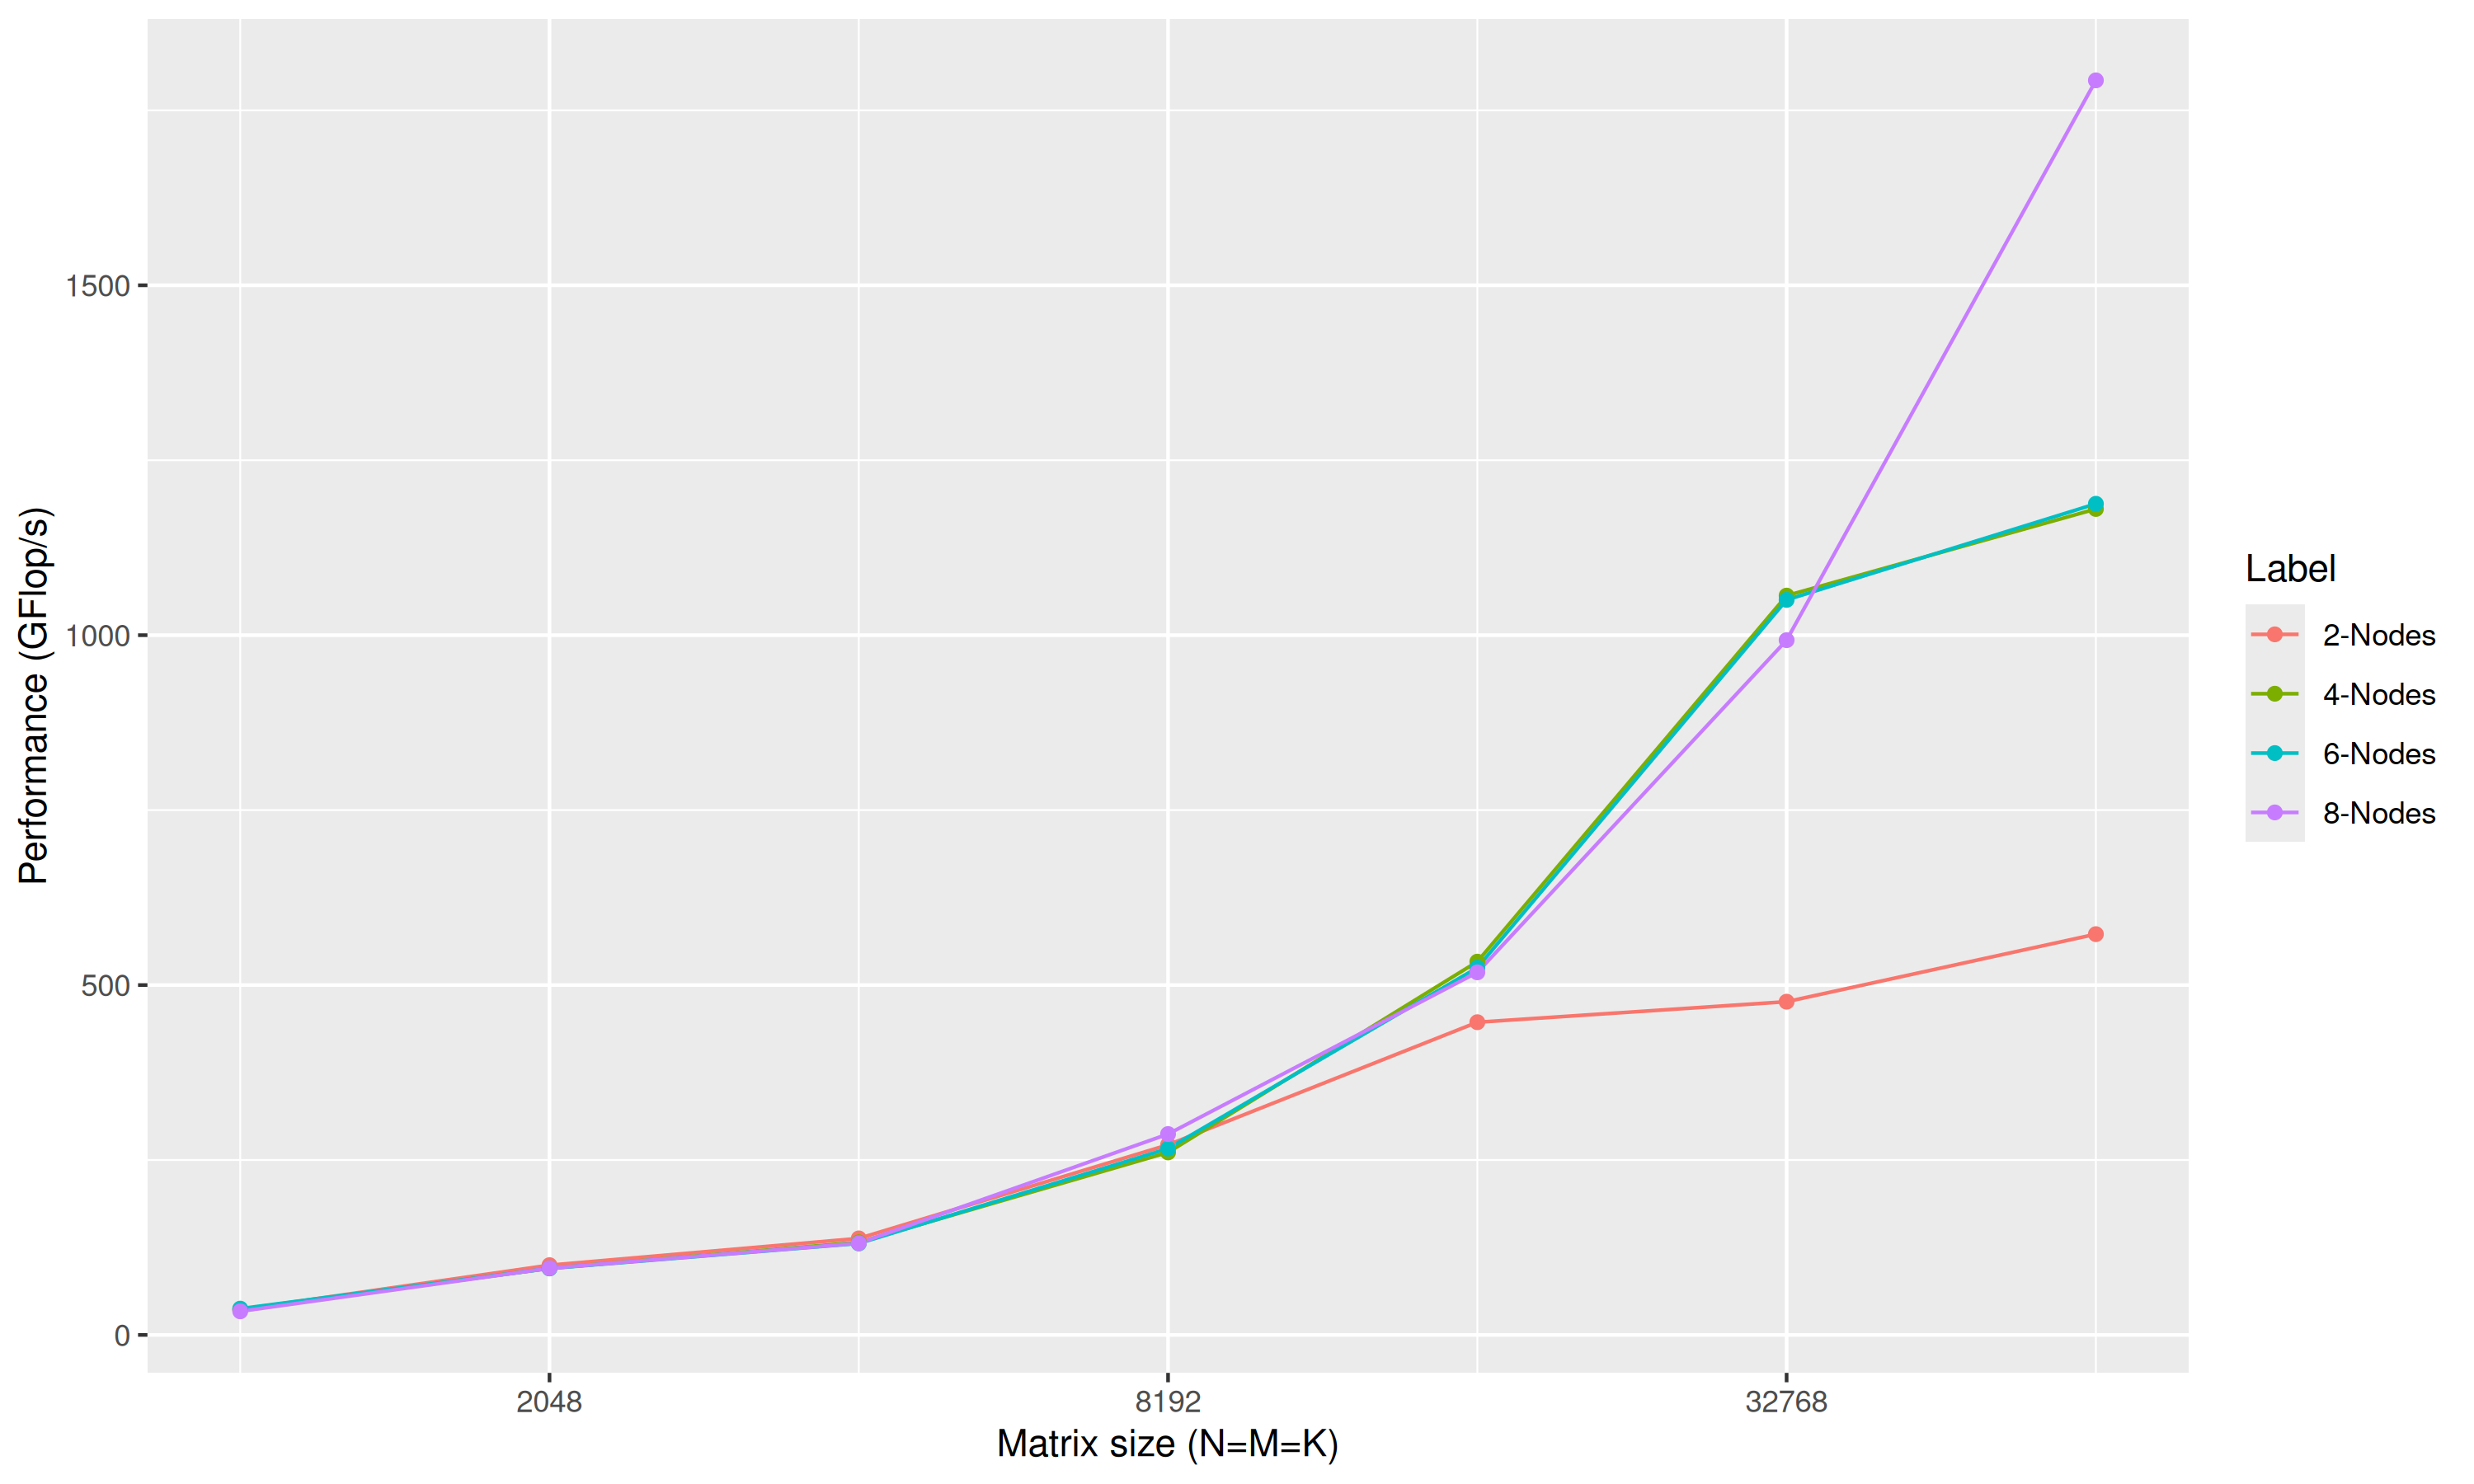
\includegraphics[width=\textwidth]{assets/dgemm_mpi/strong_summa.png}
        \caption{Test de scalabilité forte SUMMA (sans tuilage intra processus) sur plusieurs nombres nœuds}
        \label{fig:strong_summa}    
    \end{minipage}
     \hfill
    \begin{minipage}{0.48\textwidth}
        \centering
        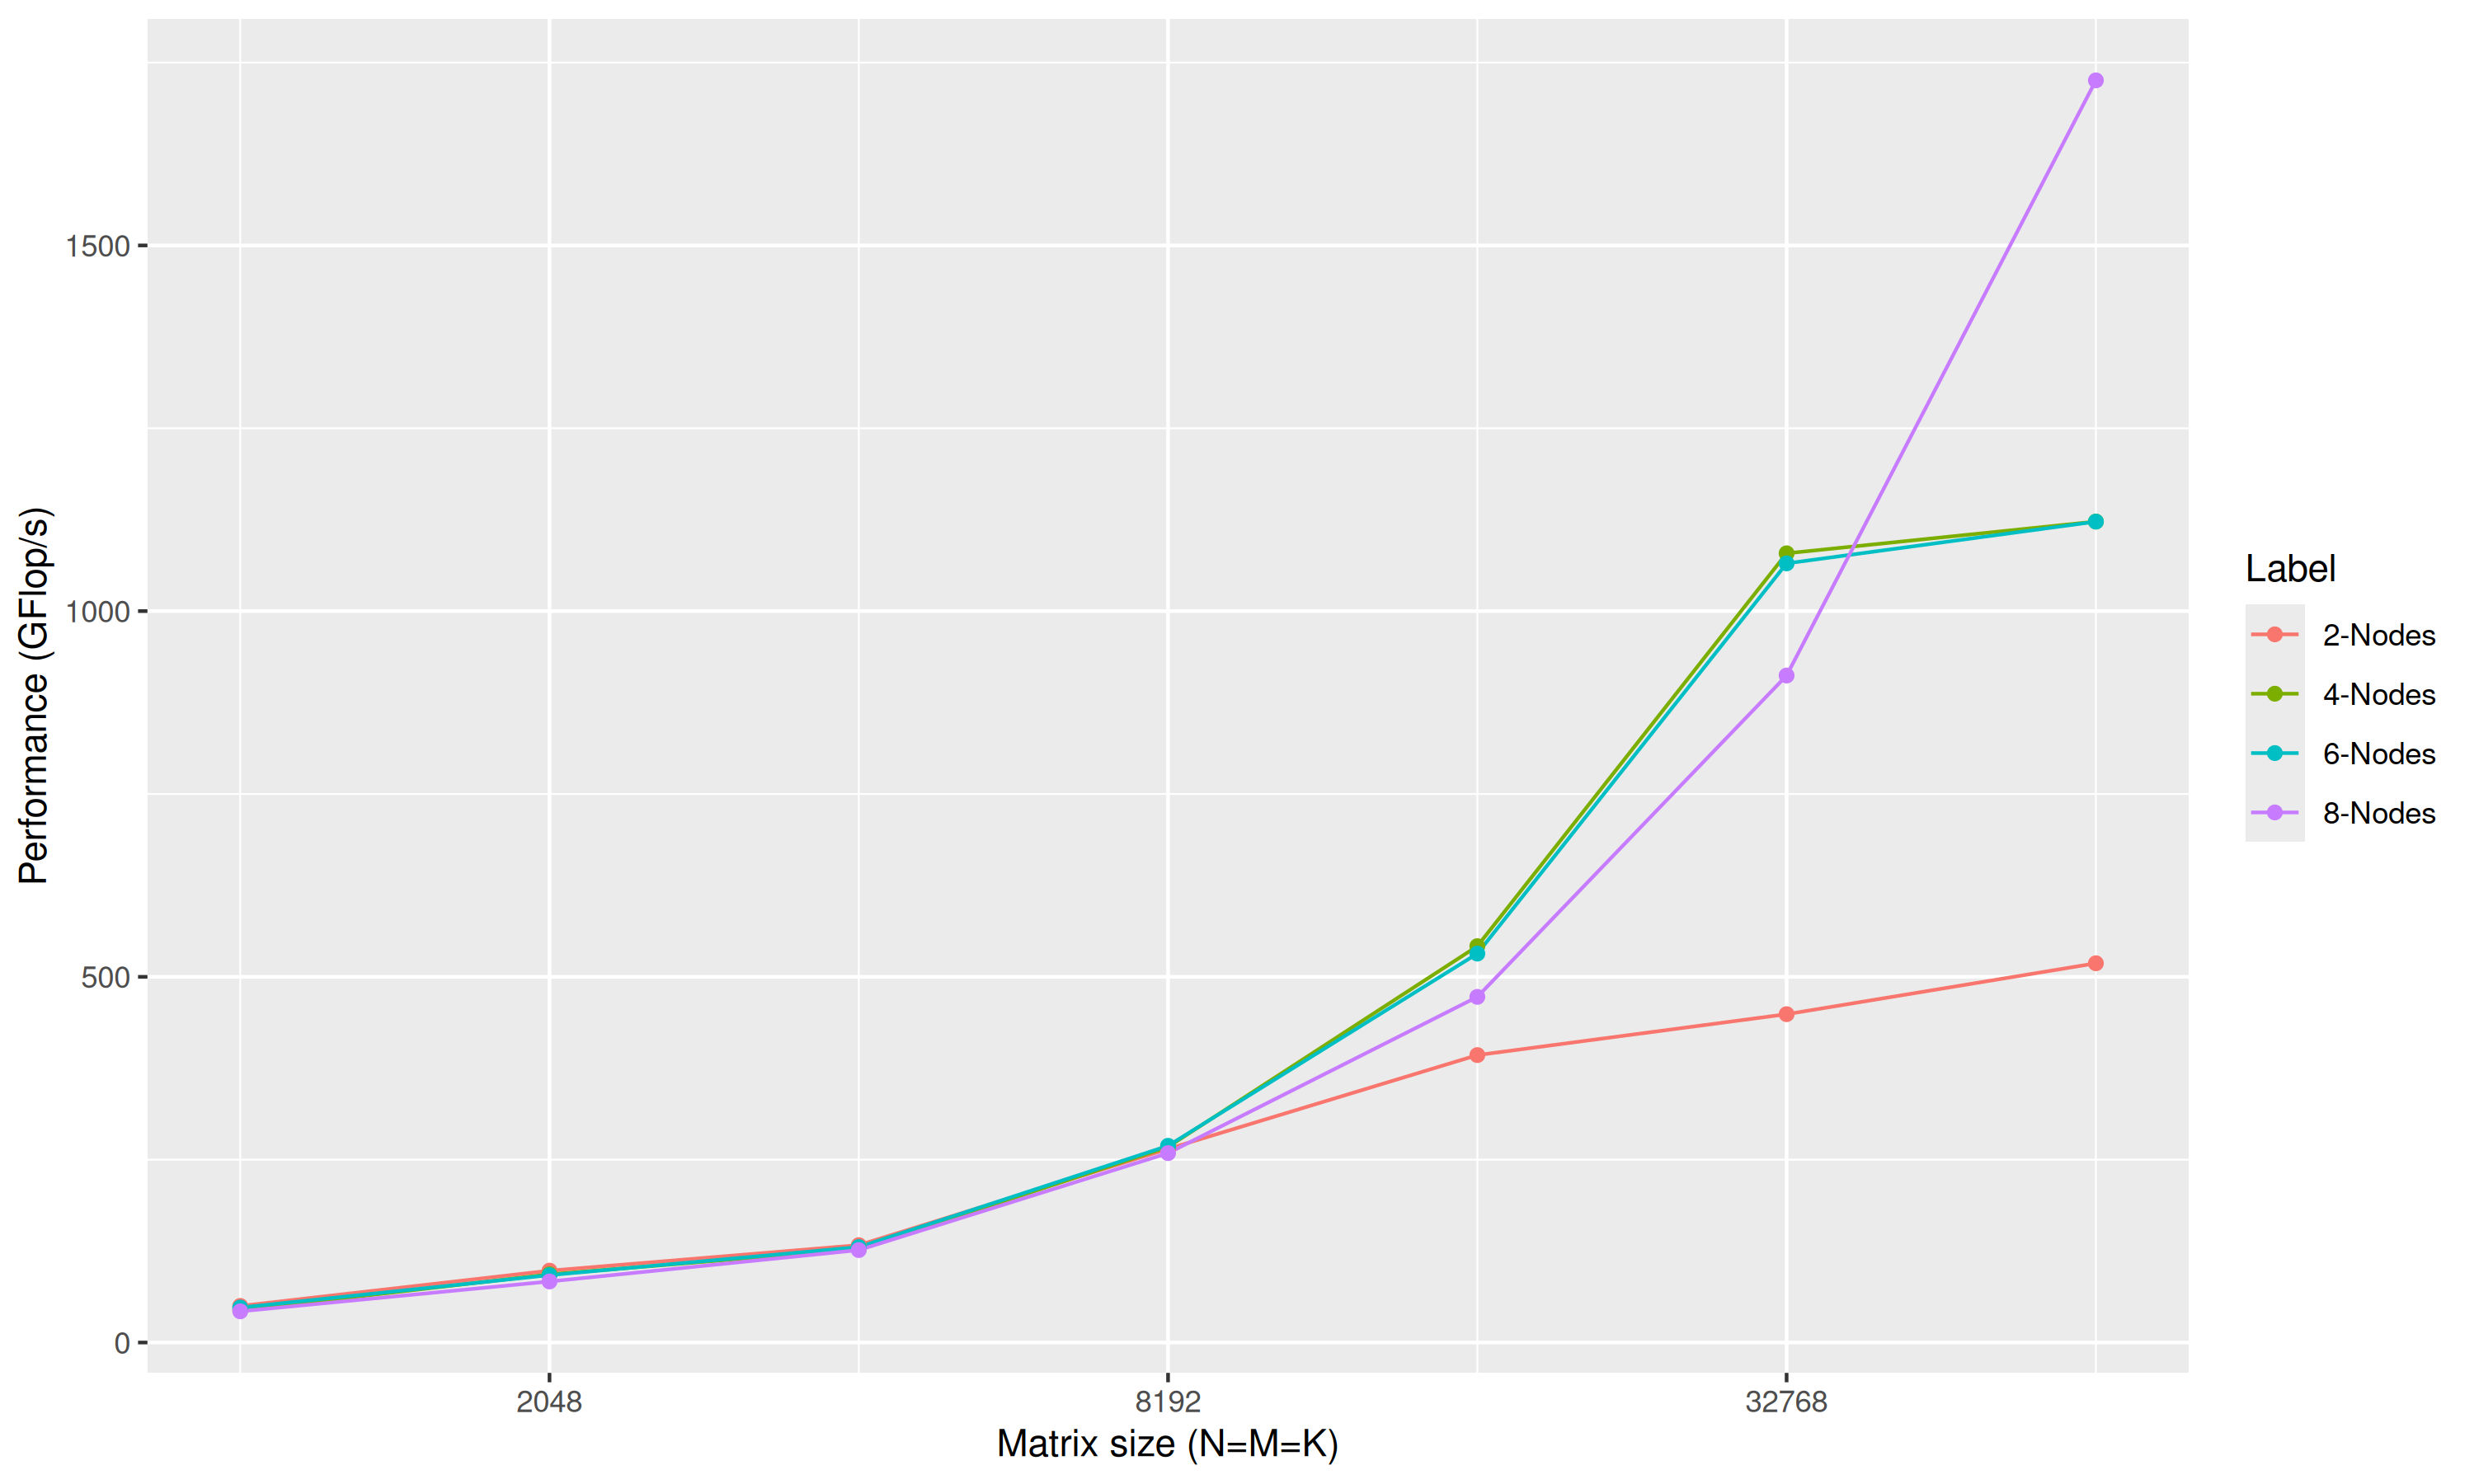
\includegraphics[width=\textwidth]{assets/dgemm_mpi/strong_opt.png}
        \caption{Test de scalabilité forte SUMMA-opt (avec tuilage intra processus) sur plusieurs nombres nœuds}
        \label{fig:strong_opt}    
    \end{minipage}

\end{figure}


Les Figures \ref{fig:strong_summa} et \ref{fig:strong_opt} permettent de comparer les performances des deux versions implémentées sur différentes tailles de matrices et nombre
de machines. Si les deux versions ont des résultats similaires sur de petites tailles de matrices, on remarque que des différences importantes (allant jusqu'à $\approx 100$Gflop/s)
commencent à apparaître à partir de 32768x32768. Ces graphiques permettent également de voir qu'utiliser un plus grand nombre de machines est plus intéressant seulement à partir de 
certains paliers. En effet, on voit que l'utilisation de 4 machines n'est réellement utile qu'avec des matrices de taille minimum 32768x32768 et qu'il en est de même avec 8 machines.
Il faut ici attendre des matrices 65536x65536 pour que la différence de performances soit intéressante.

\begin{figure}
    \centering
    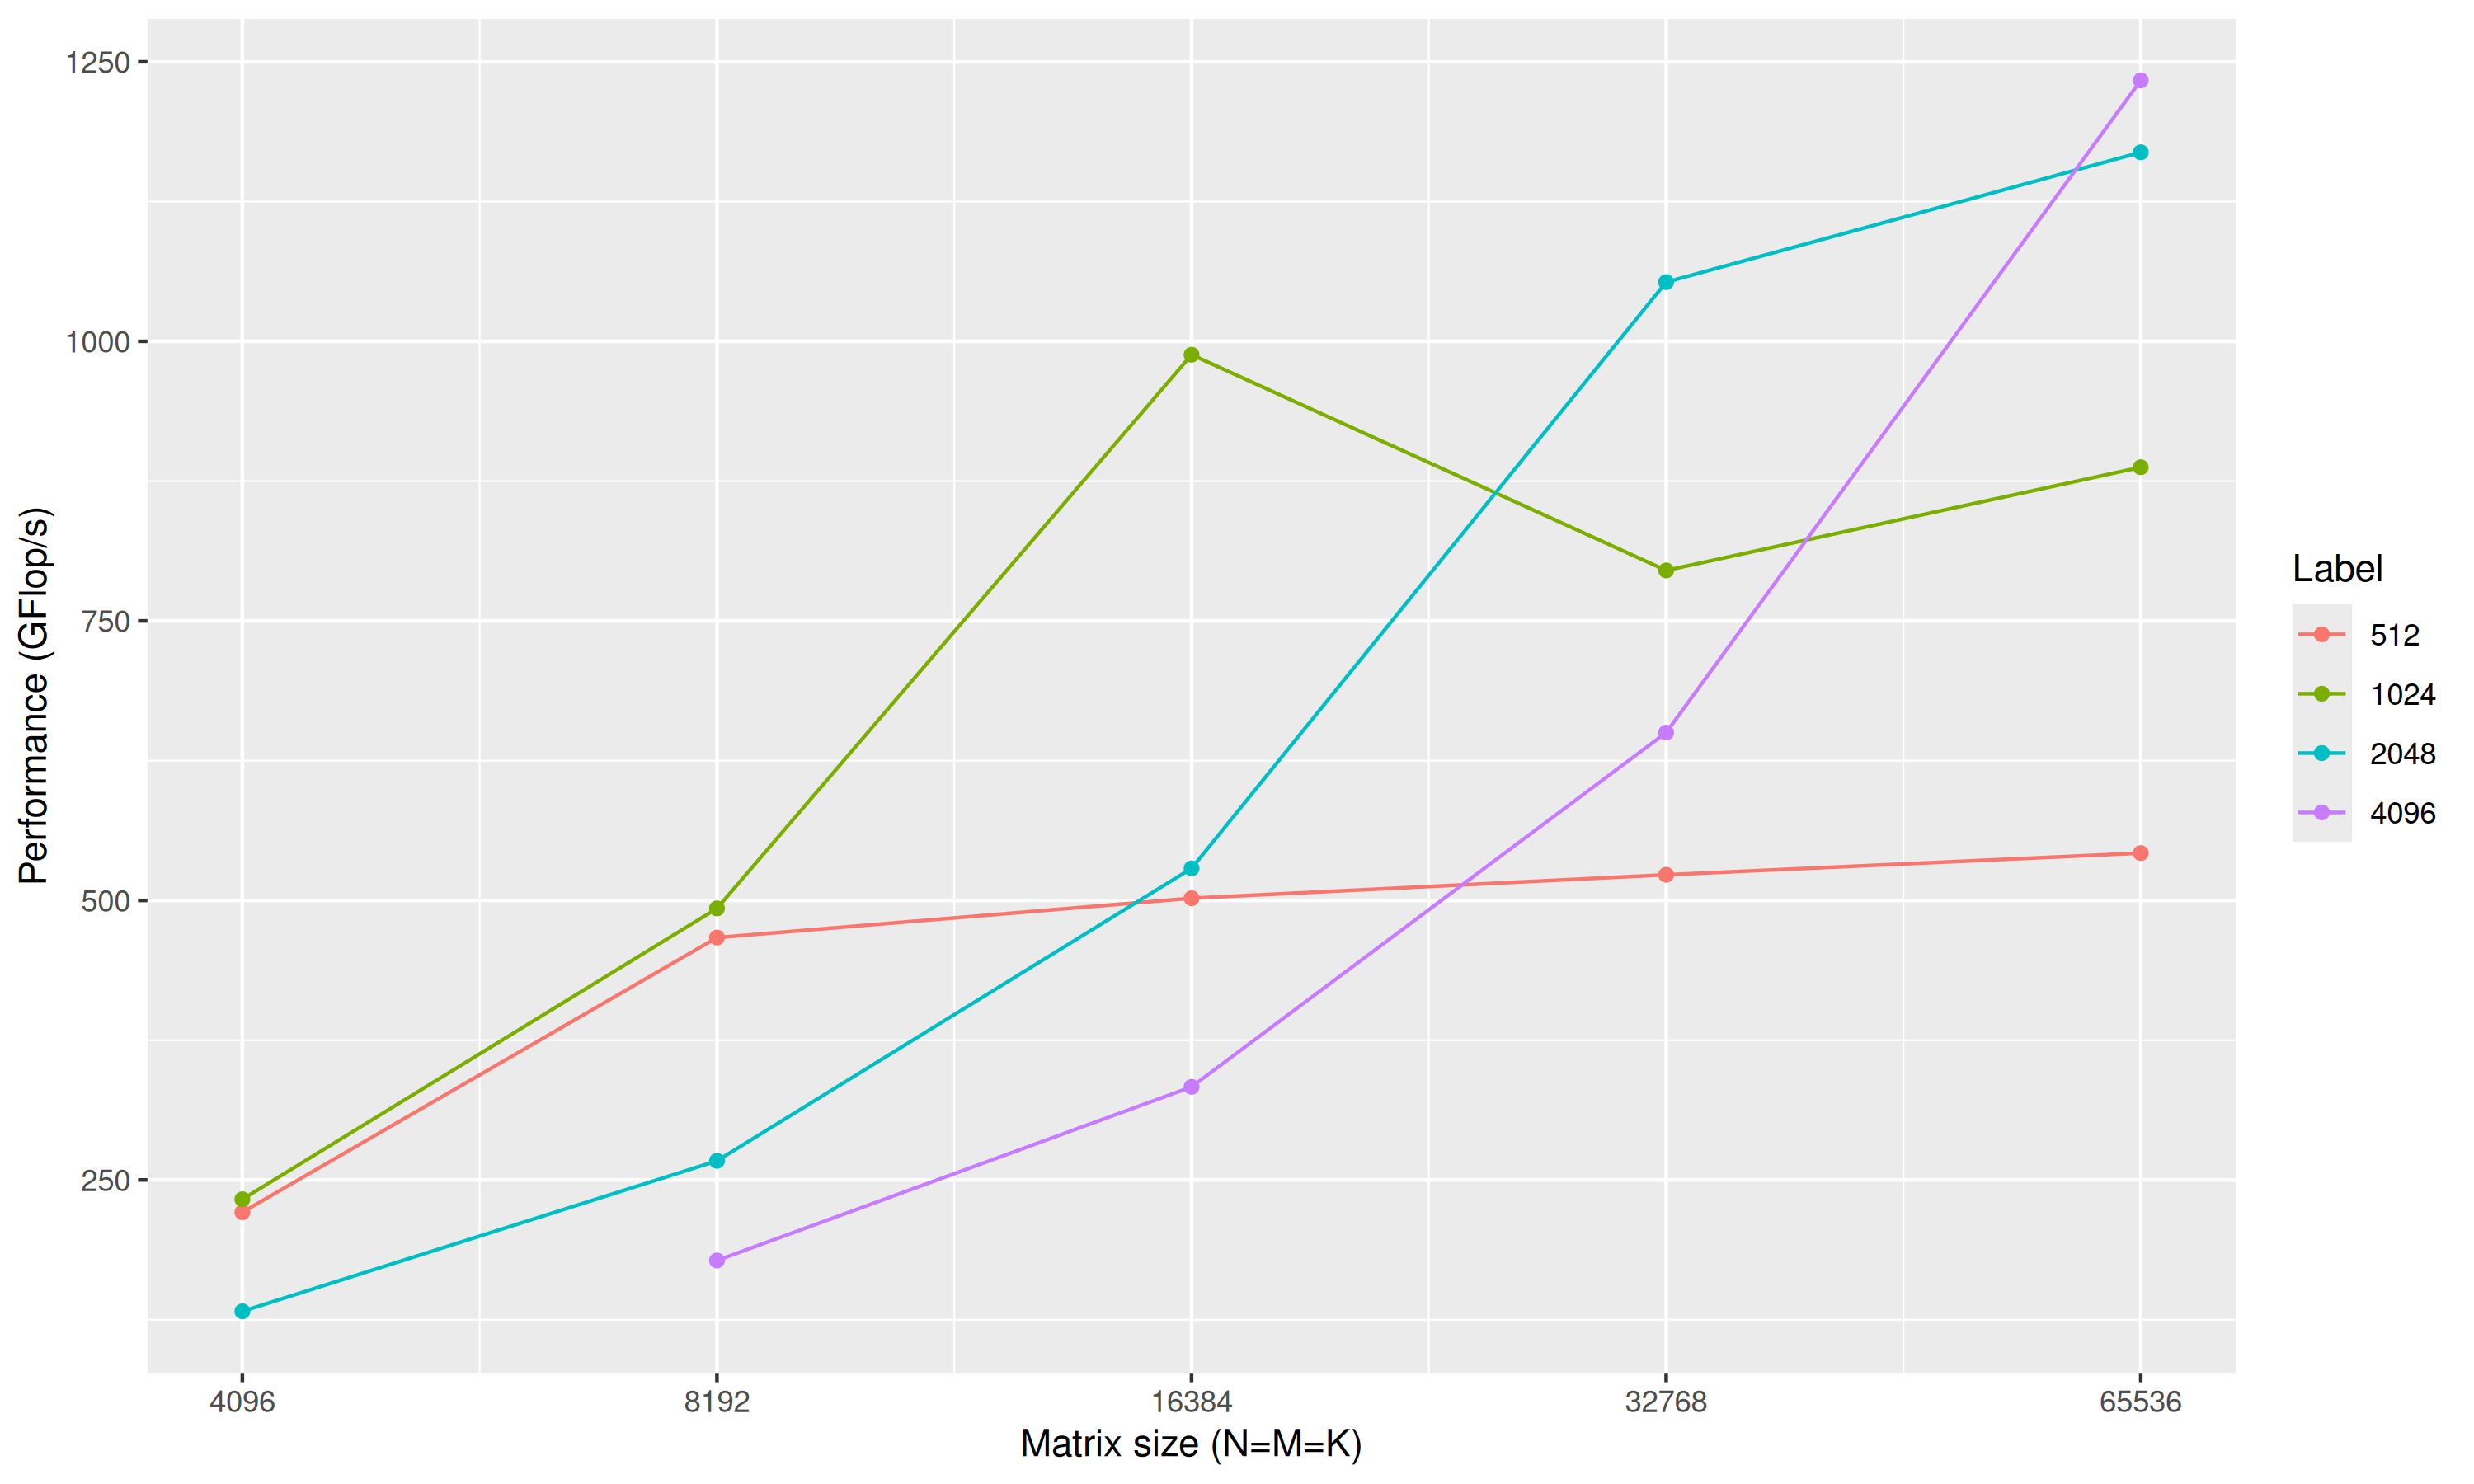
\includegraphics[width=0.8\textwidth]{assets/dgemm_mpi/block_size.png}
    \caption{Comparaison des performances en fonction de la taille des tuiles}
    \label{fig:block_size_mpi}
\end{figure}


Cette version MPI rajoute donc un nouveau paramètre à calibrer. L'espace de recherche étant bien plus grand qu'en mémoire partagée, nous avons choisi de fixer la taille
d'une tuile OpenMP à 128x128 pour la version utilisant la version tuilée. Nous avons ensuite voulu savoir quelle taille de tuile choisir, mais également l'impact que celle-ci pourrait 
avoir sur les performances. La Figure \ref{fig:block_size_mpi} représente le choix de différentes tailles de tuiles sur des tailles de matrices croissantes. Il n'est pas étonnant 
de voir que les tuiles de grandes tailles ont de meilleures performances sur les grandes matrices. Cependant, cela montre que l'on a peut être un problème de granularité car si la taille 
des tuiles à transmettre augmente aussi rapidement, on se retrouvera fortement bridés par les communications réseau.

\begin{figure}
    \centering
    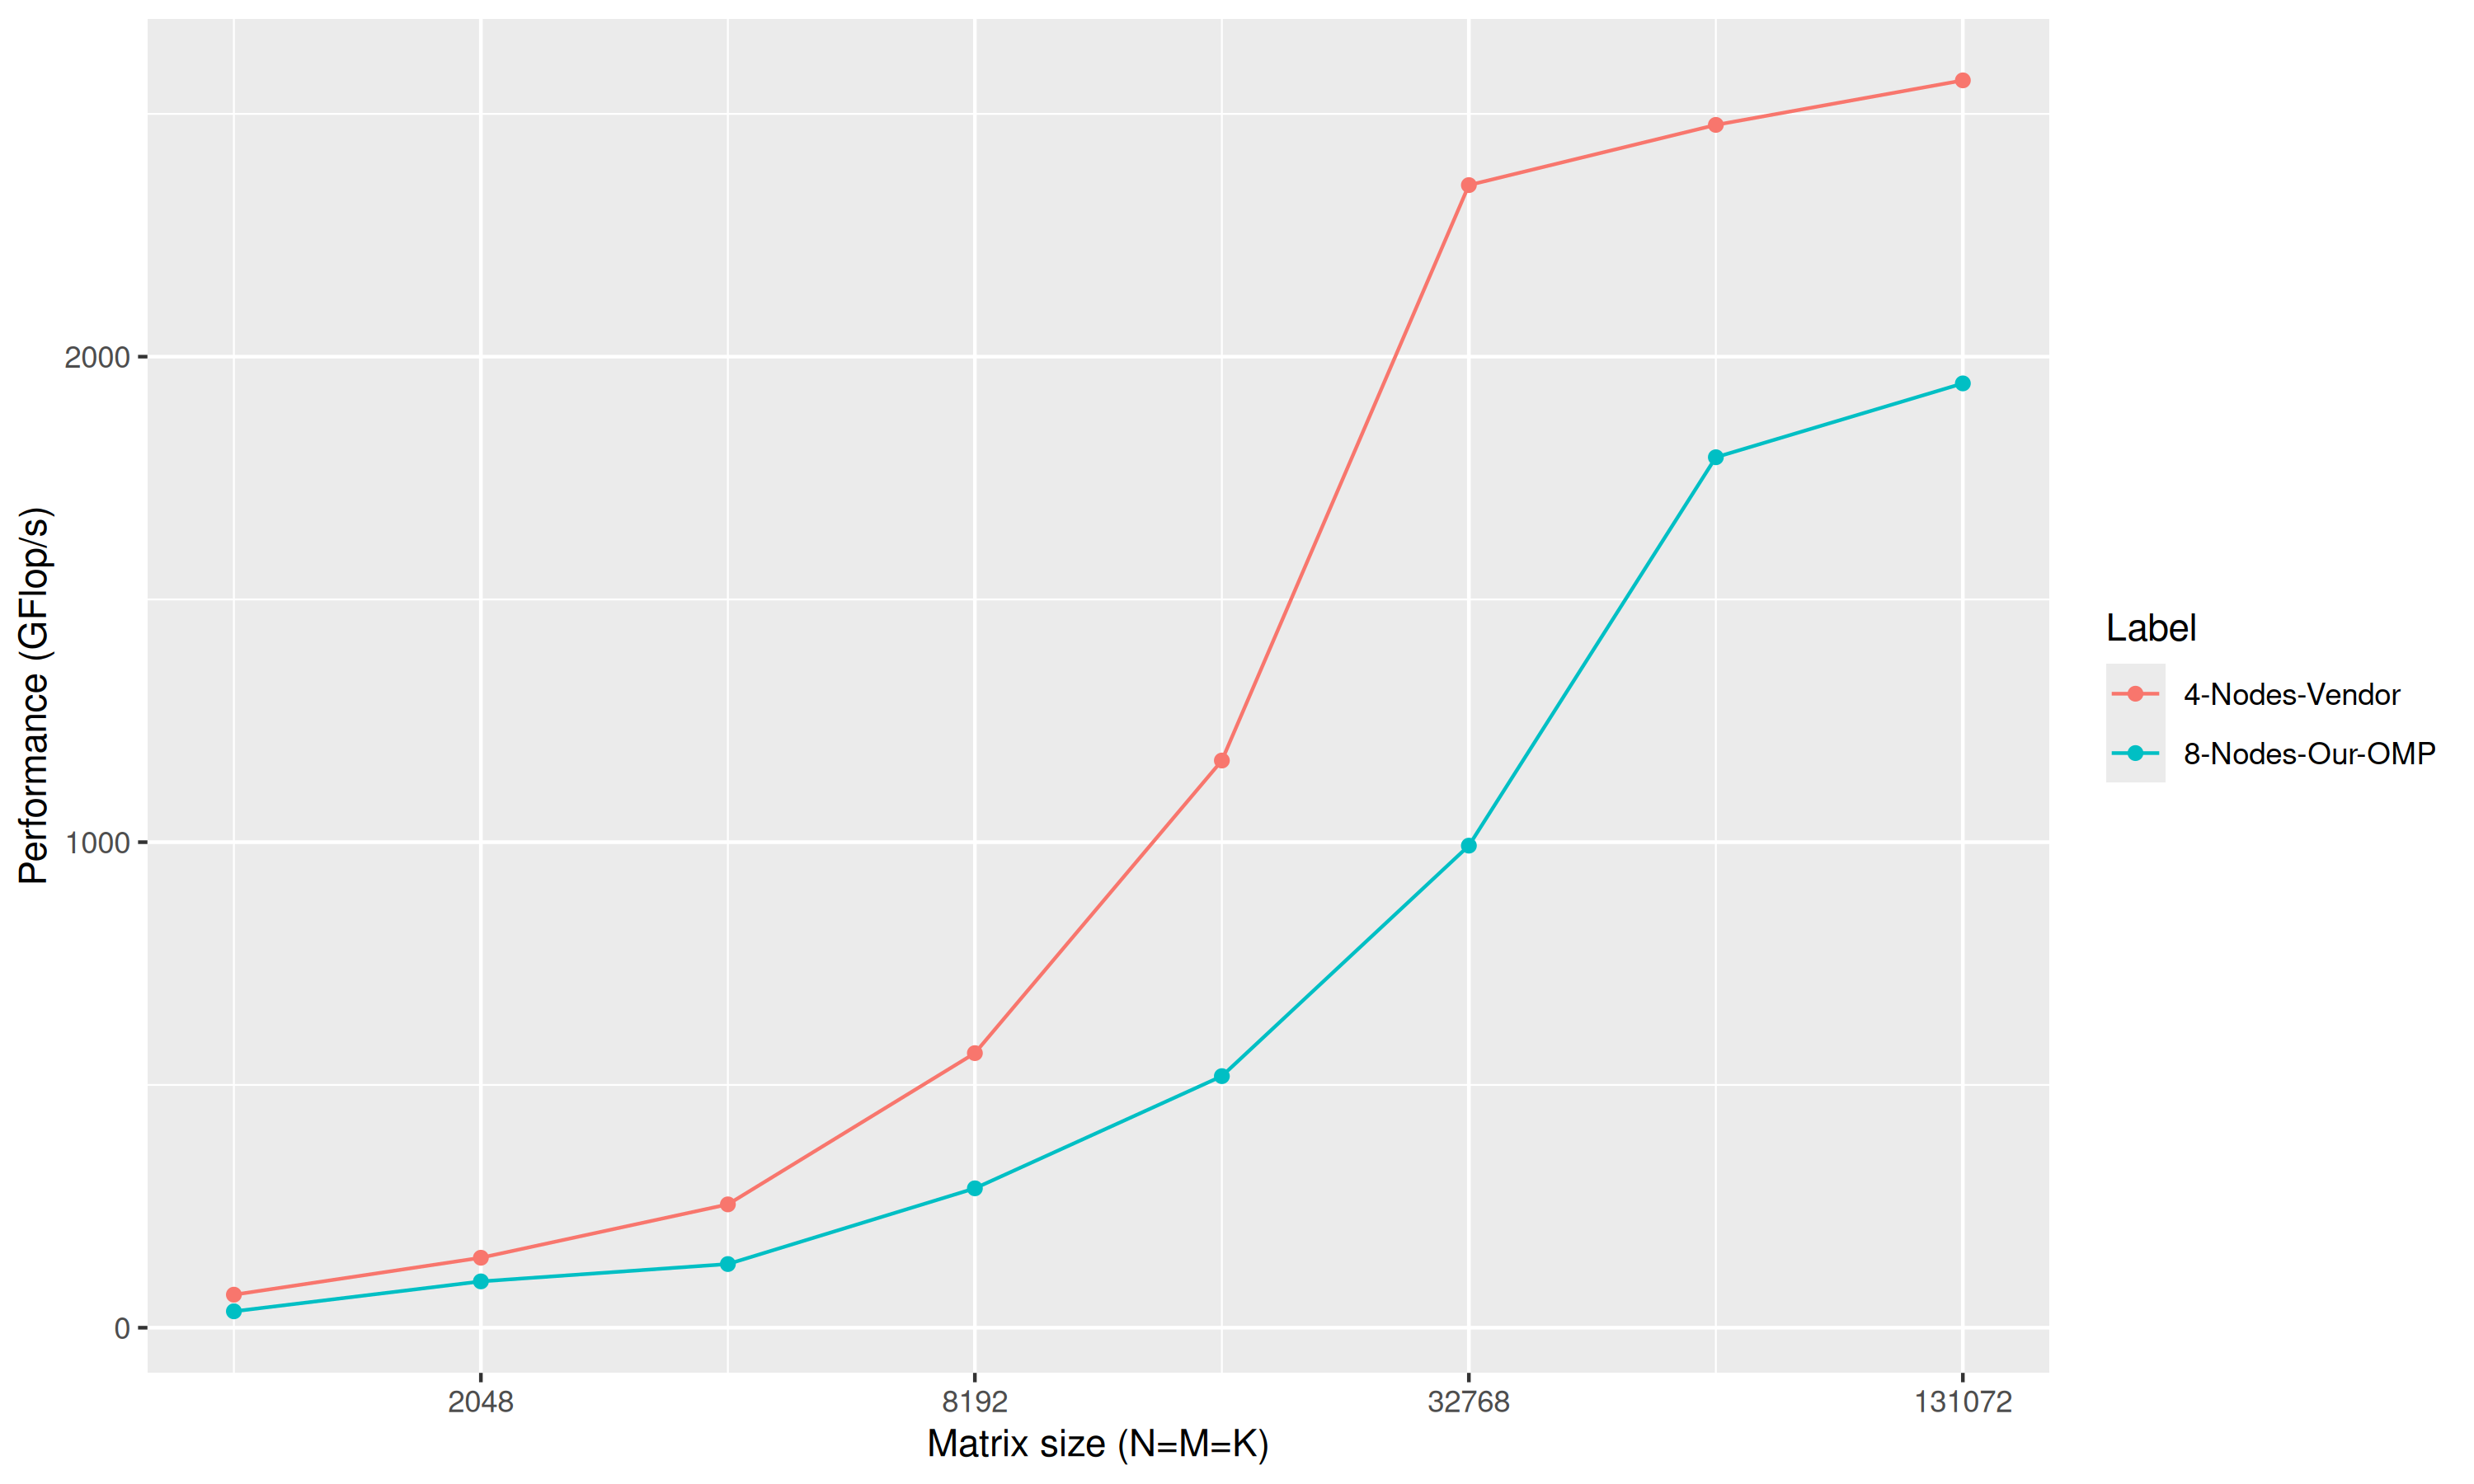
\includegraphics[width=1\textwidth]{assets/dgemm_mpi/strong_vendor.png}
    \caption{Test de scalabilité forte entre notre implémentation OpenMP (8 machines) et l'implémentation de \textit{CBLAS} (4 machines)}
    \label{fig:strong_vendor}
\end{figure}
\FloatBarrier
Comme nous savons que notre version en mémoire partagée est moins performante que celle de \textit{CBLAS}, nous avons ajouté une version ou l'appel au \textit{gemm} local se fait avec 
la version Vendor. Cela va permettre de voir les performances que l'on pourrait atteindre avec une version OpenMP plus performante. Sur la Figure \ref{fig:strong_vendor}, on remarque
un fort écart de performances notamment car la version vendor utilise 2 fois moins de machines. Ces résultats sont principalement dûs au fait que l'on ne puisse pas utiliser de manière
efficace notre version tuilée (qui donne des résultats bien plus proche de \textit{CBLAS}). Nous parvenons tout de même à presque atteindre les 2 TFlop/s sur des matrices de taille
131072x131072. 